% This work is made available under the terms of the
% Creative Commons Attribution-ShareAlike 4.0 license,
% http://creativecommons.org/licenses/by-sa/4.0/.

\documentclass[a4paper]{book}

\usepackage{wrapfig}
\usepackage{graphicx}
\usepackage{hyperref}
\usepackage{multirow}
\usepackage{scalefnt}
\usepackage{tikz}

% watermark -- for draft stage
%\usepackage[firstpage]{draftwatermark}
%\SetWatermarkLightness{0.9}
%\SetWatermarkScale{5}

% Copyright (c) 2009 by the University of Waikato, Hamilton, NZ. 
% This work is made available under the terms of the 
% Creative Commons Attribution-ShareAlike 4.0 license,
% http://creativecommons.org/licenses/by-sa/4.0/.
%
% Version: $Revision: 5479 $

\newenvironment{tight_itemize}{
\begin{itemize}
  \setlength{\itemsep}{1pt}
  \setlength{\parskip}{0pt}
  \setlength{\parsep}{0pt}}{\end{itemize}
}

\newenvironment{tight_enumerate}{
\begin{enumerate}
  \setlength{\itemsep}{1pt}
  \setlength{\parskip}{0pt}
  \setlength{\parsep}{0pt}}{\end{enumerate}
}

% if you just need a simple heading
% Usage:
%   \heading{the text of the heading}
\newcommand{\heading}[1]{
  \vspace{0.3cm} \noindent \textbf{#1} \newline
}

\newcommand{\icon}[1]{\tikz[baseline=-3pt]\node[inner sep=0pt,outer sep=0pt]{\includegraphics[height=1.1em]{#1}};}


\title{
  \textbf{ADAMS} \\
  {\Large \textbf{A}dvanced \textbf{D}ata mining \textbf{A}nd \textbf{M}achine
  learning \textbf{S}ystem} \\
  {\Large Module: adams-audio} \\
  \vspace{1cm}
  
\includegraphics[width=2cm]{images/audio-module.png} \\
}
\author{
  Peter Reutemann
}

\setcounter{secnumdepth}{3}
\setcounter{tocdepth}{3}

\begin{document}

\begin{titlepage}
\maketitle

\thispagestyle{empty}
\center
\begin{table}[b]
	\begin{tabular}{c l l}
		\parbox[c][2cm]{2cm}{\copyright 2018-2020} &
		\parbox[c][2cm]{5cm}{
\includegraphics[width=5cm]{images/coat_of_arms.pdf}} \\
	\end{tabular}
	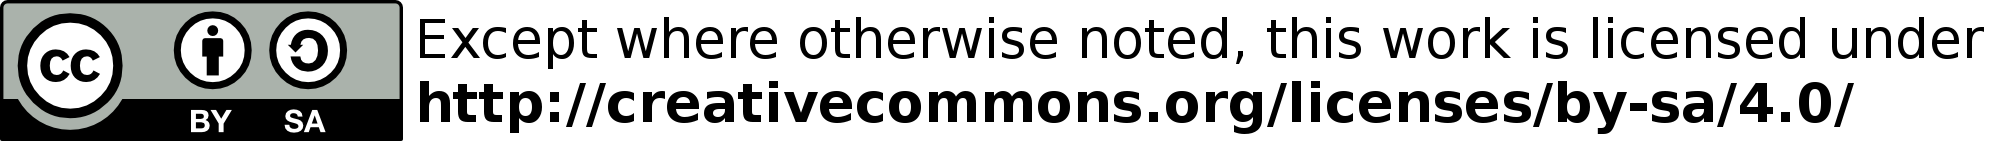
\includegraphics[width=12cm]{images/cc.png} \\
\end{table}

\end{titlepage}

\tableofcontents
%\listoffigures
%\listoftables

%%%%%%%%%%%%%%%%%%%%%%%%%%%%%%%%%%%
\chapter{Introduction}
The \textit{adams-audio} module offers some basic audio processing functionality,
like extracting information from audio files and reading their data.

There are some very good, open-source tools for processing audio:
\begin{tight_itemize}
  \item \textit{ffmpeg}\cite{ffmpeg} -- command-line tool, swiss army knife
  for audio and video processing (extraction and conversion).
  \item \textit{Audacity}\cite{audacity} -- user interface for recording and
  editing multi-track audio files.
\end{tight_itemize}


%%%%%%%%%%%%%%%%%%%%%%%%%%%%%%%%%%%
\chapter{Flow}
The following sources are available:
\begin{tight_itemize}
  \item \textit{AudioRecorder} -- records audio using the specified recorder.
  \item \textit{NewAudioAnnotations} -- creates an empty audio trail data structure.
\end{tight_itemize}

\noindent The following transformers are available:
\begin{tight_itemize}
  \item \textit{AddAudioAnnotation} -- adds an audio annotation.
  \item \textit{AudioData} -- reads the data from an audio source, eg a file
  \item \textit{AudioInfo} -- generates information about an audio source
  \item \textit{AudioAnnotationsFileReader} -- reads audio annotations from disk.
  \item \textit{AudioAnnotationsFileWriter} -- writes audio annotations to disk.
  \item \textit{AudioAnnotationsFilter} -- applies a filter to an audio annotations.
  \item \textit{WaveFeatureGenerator} -- generates features from a Wave object
  using the specified generator
  \item \textit{WaveFilter} -- applies the specified filter to the Wave object.
\end{tight_itemize}

\noindent The following sinks are available:
\begin{tight_itemize}
  \item \textit{AudioPlayback} -- can playback audio files (e.g., MP3 or Wave).
  \item \textit{MP3ToWave} -- converts MP3 files to Wave ones.
\end{tight_itemize}

\noindent The following Wave filters are available:
\begin{tight_itemize}
  \item \textit{Cut} -- Cuts out a portion of the Wave object
  \item \textit{PassThrough} -- dummy, does nothing
  \item \textit{Resample} -- resample the amplitudes to a new sample rate
  \item \textit{Trim} -- removes data left and right
\end{tight_itemize}

\noindent The following conversions are available:
\begin{tight_itemize}
  \item \textit{SpectrogramToBufferedImage} -- turns a spectrogram into an image
  \item \textit{WaveToAmplitudes} -- extracts the amplitudes from a Wave object
  \item \textit{WaveToSpectrogram} -- generates a spectrogram from a Wave object
\end{tight_itemize}

\noindent The following Wave feature generators are available:
\begin{tight_itemize}
  \item \textit{Fingerprint}
  \item \textit{Histogram}
  \item \textit{Spectrogram}
\end{tight_itemize}

\section{Spectrograms}
There are currently two ways of generating spectrogram output:
\begin{tight_itemize}
  \item image
  \item tabular data
\end{tight_itemize}

\noindent In order to generate an \textit{image} of a spectrogram, you need to:
\begin{tight_itemize}
  \item turn the \textit{Wave} container into a spectrogram data structure,
  using the \textit{WaveToSpectrogram} conversion
  \item turn the \textit{Spectrogram} data structure into an image using
  the \textit{SpectrogramToBufferedImage} conversion
\end{tight_itemize}
Example flow \textit{adams-audio-wav\_spectrogram\_image.flow} incorporates
these steps and Figure \ref{spectrogram} shows the generated example image.

\begin{figure}[htb]
  \centering
  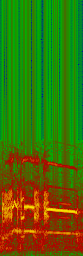
\includegraphics[width=4.0cm]{images/spectrogram.png}
  \caption{Spectrogram with gradient using multiple colors.}
  \label{spectrogram}
\end{figure}

\clearpage
\noindent If you want to generated \textit{tabular data} from a spectrogram,
you need to:
\begin{tight_itemize}
  \item generate features from the \textit{Wave} container using the
  \textit{WaveFeatureGenerator} transformer with the \textit{Spectrogram}
  feature generator
  \item what kind of output is being generated, is determined by the
  \textit{converter} that is part of the feature generator
\end{tight_itemize}
Example flow \textit{adams-audio-wav\_spectrogram.flow} shows how to do this.

%%%%%%%%%%%%%%%%%%%%%%%%%%%%%%%%%%%
\chapter{Conversion}
Since the \textit{adams-audio} module is limited to using WAV (aka PCM) files,
you need to convert other audio formats first. You can do this, either on
the command-line outside ADAMS (e.g., using ffmpeg or avconv natively), or
using the \textit{FFmpeg} sink actor. The latter provides a wrapper around
ffmpeg/avconv.

Here is an example command-line conversion of an MP3 file into a WAV one, using
ffmpeg:
\begin{verbatim}
ffmpeg -i sample.mp3 -acodec pcm_s16le -ar 44100 sample.wav
\end{verbatim}

Use the following command-line to list all the available \textit{encoders}
that are available on your system:
\begin{verbatim}
ffmpeg -encoders
\end{verbatim}

\section{Audio filters}
\textit{ffmpeg} can be used to apply audio filters as well. See the following
website for more details: \\

\url{http://www.ffmpeg.org/ffmpeg-filters.html#Audio-Filters}{}

%%%%%%%%%%%%%%%%%%%%%%%%%%%%%%%%%%%
% Copyright (c) 2009-2012 by the University of Waikato, Hamilton, NZ. 
% This work is made available under the terms of the 
% Creative Commons Attribution-ShareAlike 4.0 license,
% http://creativecommons.org/licenses/by-sa/4.0/.
%
% Version: $Revision$

\begin{thebibliography}{999}
	% to make the bibliography appear in the TOC
	\addcontentsline{toc}{chapter}{Bibliography}

    % references
	\bibitem{adams}
		\textit{ADAMS} -- Advanced Data mining and Machine learning System \\
		\url{https://adams.cms.waikato.ac.nz/}{}
		
	\bibitem{heatmap}
		\textit{Heat map} -- WikiPedia article \\
		\url{http://en.wikipedia.org/wiki/Heat_map}{}

\end{thebibliography}


\end{document}
